\chapter{Pixelové detektory radiace}
\label{kap:2}
%TODO Pixelove detektory radiace Timepix? nebo nechat obecne?
Mezi možnosti detekovat ionizující záření patří mimo jiné, použití pixelových detektorů. Pomocí pixelových detektorů, konkrétněji hybridních pixelových detektorů, jsme schopni detailně změřit ionizující záření, které interaguje s detektorem. V dalších částech této kapitoly bude popsána obecná činnost a princip detekce radiace pixelových detektorů. V kapitole \ref{kap:3}, bude konkrétně popsán detektor z rodiny Timepix \cite{Llopart}, konkrétněji detektor Timepix 2 \cite{tpx2_manual}. 


\section{Princip činnosti pixelových detektorů}
\label{kap:2.1}
V této části bude popsán obecný princip činnosti společný pro detektory radiace z rodiny Timepix \cite{Llopart}, vyvíjenými pod záštitou CERN Medpipix Collaboration \cite{Medpix}. Pixelový detektor, přesněji hybridní pixelový detektor se skládá ze dvou oddělitelných částí, ze senzorové vrstvy a vrstvy s vyčítací elektronikou viz. obrázek \ref{fig:Timepix}. Právě toto rozdělení na senzorovou a vyčítací část označuje název hybridní detektor.
\par Senzorová vrstva je tvořena polovodičovým materiálem. Důležitými parametry senzorové vrstvy jsou typ polovodičového materiálu a její tloušťka. Nejčastěji používané materiály jsou $\text{Si}$, $\text{CdTe}$ a $\text{GaAs}$. % TODO reference materialy.
Na senzorovou vrstvu je připojené vysoké napětí, označované jako \textit{bias voltage}. Toto vysoké napětí zajistí vyprázdnění oblasti v polovodičové struktuře senzorové vrstvy. Pokud částice ionizujícího záření interaguje v senzorové vrstvě, dojde k vytvoření náboje. Tento náboj je dále zpracován vyčítací elektronikou která je pomocí technologie nazývající se \textit{bump bond}, připojena k senzorové vrstvě.
\par Vyčítací vrstva (ASIC) je rozdělena na 256x256 individuálních pixelů. Každý pixel obsahuje potřebnou elektroniku ke zpracovaní náboje, vzniklého v senzorové vrstvě. Detailnější popis zpracování signálu na úrovni jednotlivých pixelů, bude popsán pro konkrétní pixelový detektor Timepix 2 v kapitole \ref{kap:3}. Signál po zpracování v jednotlivých pixelech digitální společnou částí vyčítací vrstvy převeden na výstupní plošky. Vyčítací vrstva je poté pomocí \textit{wire bond} technologie připojena k desce plošných spojů. Signály vedoucí z pixelových detektorů jsou následně zpracovány vyčítacím zařízením. Druhy vyčítacích zařízní budou popsány v následující části.
 \begin{figure}[h!]
 	\centering
 	\captionsetup{justification=centering}
 	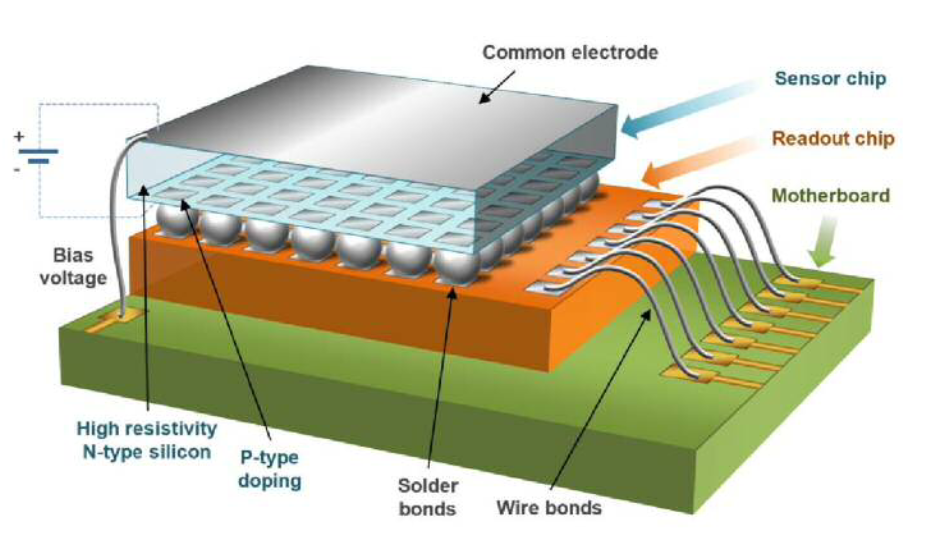
\includegraphics[scale=0.55]{Timepix.png}
 	\caption{Rozložení hybridního pixelového detektoru Timepix \cite{Platkevic}} 
 	\label{fig:Timepix}
 \end{figure}	

%\section{Druhy pixelových detektorů} %plus jejich použití	-> asi zbytečná část

\section{Vyčítací zařízení pro pixelové detektory}
Každý pixelový detektor z rodiny detektorů Timepix \cite{Llopart}, má specifické požadavky pro návrh vyčítacího zařízení. Základními požadavky jakými jsou napájecí napětí detektoru a komunikační rozhraní s detektorem, musí být vždy splněny aby bylo možné spolehlivě pracovat s pixelovým detektorem. Vyčítacíh zařízení existuje celá řada. V této práci, respektivě v následujících částech bude popsán návrh miniaturizovaného vyčítacího rozhraní. Pokusím se zde uvést příklady miniaturizovaných zařízení.
\subsection{USB Lite}
Dosud nejmenším vyčítacím zařízení rodiny detektorů Timepix \cite{Llopart}, je zařízení \textit{USB Lite} \cite{usb_lite}, viz. obrázek \ref{fig:usb_lite}. Toto zařízení umožňuje komunikovat s detektorem Medipix 2 \cite{Medpix2}. Rozměry zařízení jsou 60x15 mm. Rychlost vyčítání snímků je 4 fps a spotřeba zařízení je menší než 2 W \cite{usb_lite}.
 \begin{figure}[h!]
	\centering
	\captionsetup{justification=centering}
	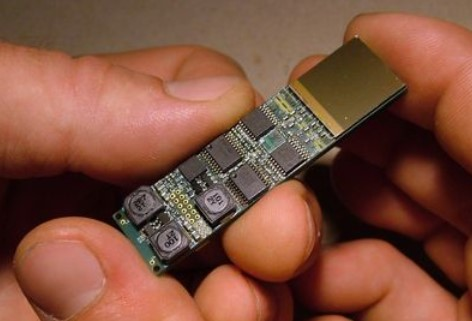
\includegraphics[scale=0.55]{usb_lite.jpg}
	\caption{Vyčítací zařízení \textit{USB lite}} 
	\label{fig:usb_lite}
\end{figure}	

\subsection{MiniPIX SPRINTER}
Vyčítací zařízení MiniPIX SPRINTER je vyvíjeno společností ADVACAM, zařízení je možné vidět na obrázku \ref{fig:sprinter}. Toto zařízení umožňuje komunikovat s detektorem Timepix 2 \cite{tpx2_manual}. Rozměry zařízení jsou 50x21x14 mm. Rychlost vyčítání snímků je 99 \cite{Advacam}.
\begin{figure}[h!]
	\centering
	\captionsetup{justification=centering}
	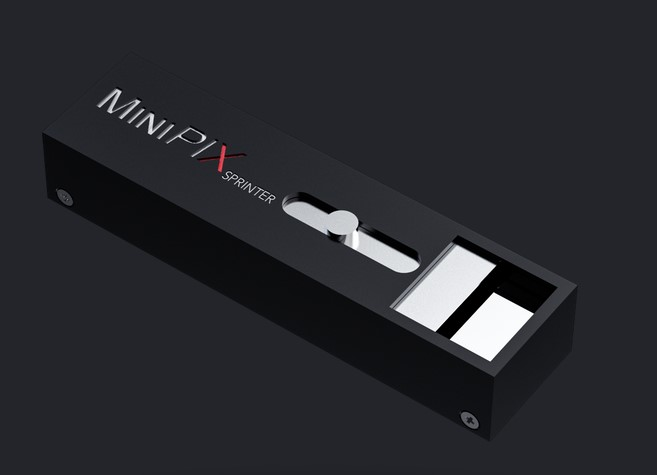
\includegraphics[scale=0.55]{sprinter.jpg}
	\caption{Vyčítací zařízení MiniPIX SPRINTER} 
	\label{fig:sprinter}
\end{figure}	

\subsection{Katherine pro Timepix 2}
Posledním uvedeným tipem vyčítacího zařízení je zařízení Kathrine pro Timepix 2 viz., obrázek \ref{fig:Katherine2}. Toto vyčítací zařízní se od předchozích dvou uvedených liší ve velikosti a rychlosti zařízení. Zařízení se skládá ze dvou částí. Samotným vyčítacím zařízením, na obrázku \ref{fig:Katherine2} v pravo a takzvaným \textit{chipboardem}, na obrázku \ref{fig:Katherine2} vlevo. Část chipboardu obstahuje detektor Timepix 2 a napájecí zdroje potřebné pro provoz detektoru. Dále jsou ze propojeny signály z konektoru od vyčítacího zařízení po samotný Timepix 2. Výhodou tohoto modulárního zapojení je možnost modifikace chipboardové části. Tedy možnost k jednomu vyčítacímu zařízení, připojit různé chipboardy. Parametry samotného vyčítacího zařízení jsou následující. Rozměry 100 x 80 x 28 mm, rychlost vyčítaní až 3.2 Gbps \cite{Burian_2020}.
\begin{figure}[h!]
	\centering
	\captionsetup{justification=centering}
	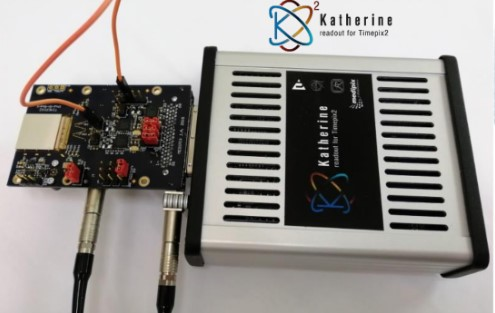
\includegraphics[scale=0.75]{Katherine2.jpg}
	\caption{Vyčítací zařízení Katherine pro Timepix 2 \cite{Burian_2020}} 
	\label{fig:Katherine2}
\end{figure}	


